\let\negmedspace\undefined
\let\negthickspace\undefined
\documentclass[journal]{IEEEtran}
\usepackage[a5paper, margin=10mm, onecolumn]{geometry}
%\usepackage{lmodern} % Ensure lmodern is loaded for pdflatex
\usepackage{tfrupee} % Include tfrupee package

\setlength{\headheight}{1cm} % Set the height of the header box
\setlength{\headsep}{0mm}     % Set the distance between the header box and the top of the text

\usepackage{gvv-book}
\usepackage{gvv}
\usepackage{cite}
\usepackage{amsmath,amssymb,amsfonts,amsthm}
\usepackage{algorithmic}
\usepackage{graphicx}
\usepackage{textcomp}
\usepackage{xcolor}
\usepackage{txfonts}
\usepackage{listings}
\usepackage{enumitem}
\usepackage{mathtools}
\usepackage{gensymb}
\usepackage{comment}
\usepackage[breaklinks=true]{hyperref}
\usepackage{tkz-euclide} 
\usepackage{listings}
% \usepackage{gvv}                                        
\def\inputGnumericTable{}                                 
\usepackage[latin1]{inputenc}                                
\usepackage{color}                                            
\usepackage{array}                                            
\usepackage{longtable}                                       
\usepackage{calc}                                             
\usepackage{multirow}                                         
\usepackage{hhline}                                           
\usepackage{ifthen}                                           
\usepackage{lscape}
\begin{document}

\bibliographystyle{IEEEtran}
\vspace{3cm}

\title{3-3.2-31}
\author{EE24BTECH11064 - Harshil Rathan}
% \maketitle
% \newpage
% \bigskip
{\let\newpage\relax\maketitle}

\renewcommand{\thefigure}{\theenumi}
\renewcommand{\thetable}{\theenumi}
\setlength{\intextsep}{10pt} % Space between text and floats


\numberwithin{equation}{enumi}
\numberwithin{figure}{enumi}
\renewcommand{\thetable}{\theenumi}
\textbf{Question}:\\
A triangle $ABC$ can be constructed $\angle{B}$ = $60^\circ$, $\angle{C}$=$45^\circ$ and $AB+BC+CA=12$cm.
\\
\solution \\
\begin{table}[h!]
    \centering
    \begin{tabular}[12pt]{ |c| c|}
    \hline
    \textbf{Equations}& \textbf{Given}\\ 
    \hline
     $2y$ & $3x+12$ \\
    \hline 
     $x$ & $2, 8 $\\
    \hline
    \end{tabular}
    \caption{Given Equations}

\end{table}
Find $\angle{A}$
\begin{align}
     \angle{A}+\angle{B}+\angle{C}=180^\circ 
\end{align}    
\begin{align}    
     \angle{A}=75^\circ
\end{align}
Applying law of Sines,
\begin{align}
          \frac{AB}{\sin{75^\circ}} + \frac{BC}{\sin{60^\circ}}+\frac{CA}{\sin{45^\circ}}=K
\end{align}
It is given that 
\begin{align}
 AB+BC+CA=12
\end{align}
\begin{align}
    AB =K \sin{75^\circ}\\
    BC =K \sin{60^\circ}\\
    CA =K \sin{45^\circ}
\end{align}
\begin{align}
    K(\frac{\sqrt{6}+\sqrt{2}}{4})+K(\frac{\sqrt{3}}{2})+K(\frac{1}{\sqrt{2}})=12
\end{align}
\begin{align}
    K=\frac{48}{\sqrt{6}+2\sqrt{2}+2\sqrt{3}}
\end{align}
Possible values of AB BC CA are, 
\begin{align}
    AB = \frac{48}{\sqrt{6}+2\sqrt{2}+2\sqrt{3}}(\frac{\sqrt{6}+\sqrt{2}}{4})
\end{align}
\begin{align}
    BC = \frac{48}{\sqrt{6}+2\sqrt{2}+2\sqrt{3}}(\frac{\sqrt{3}}{2})
\end{align}
\begin{align}
    CA = \frac{48}{\sqrt{6}+2\sqrt{2}+2\sqrt{3}}(\frac{1}{\sqrt{2}})
\end{align}
\begin{figure}[h!]
   \centering
   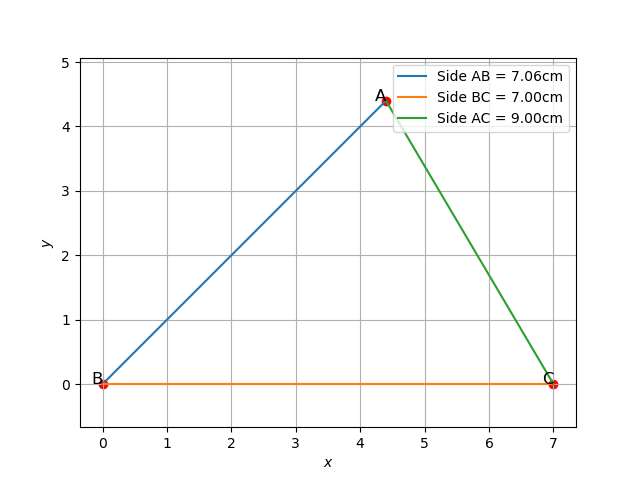
\includegraphics[width=\linewidth]{figs/Figure_1.png}
   \caption{}
   \label{stemplot}
\end{figure}





\end{document}
